
\Problem{Les fractals del poder}

\Statement

Ajudeu la Galadriel a salvar la raça èlfica conjurant les fractals del poder!

\begin{center}
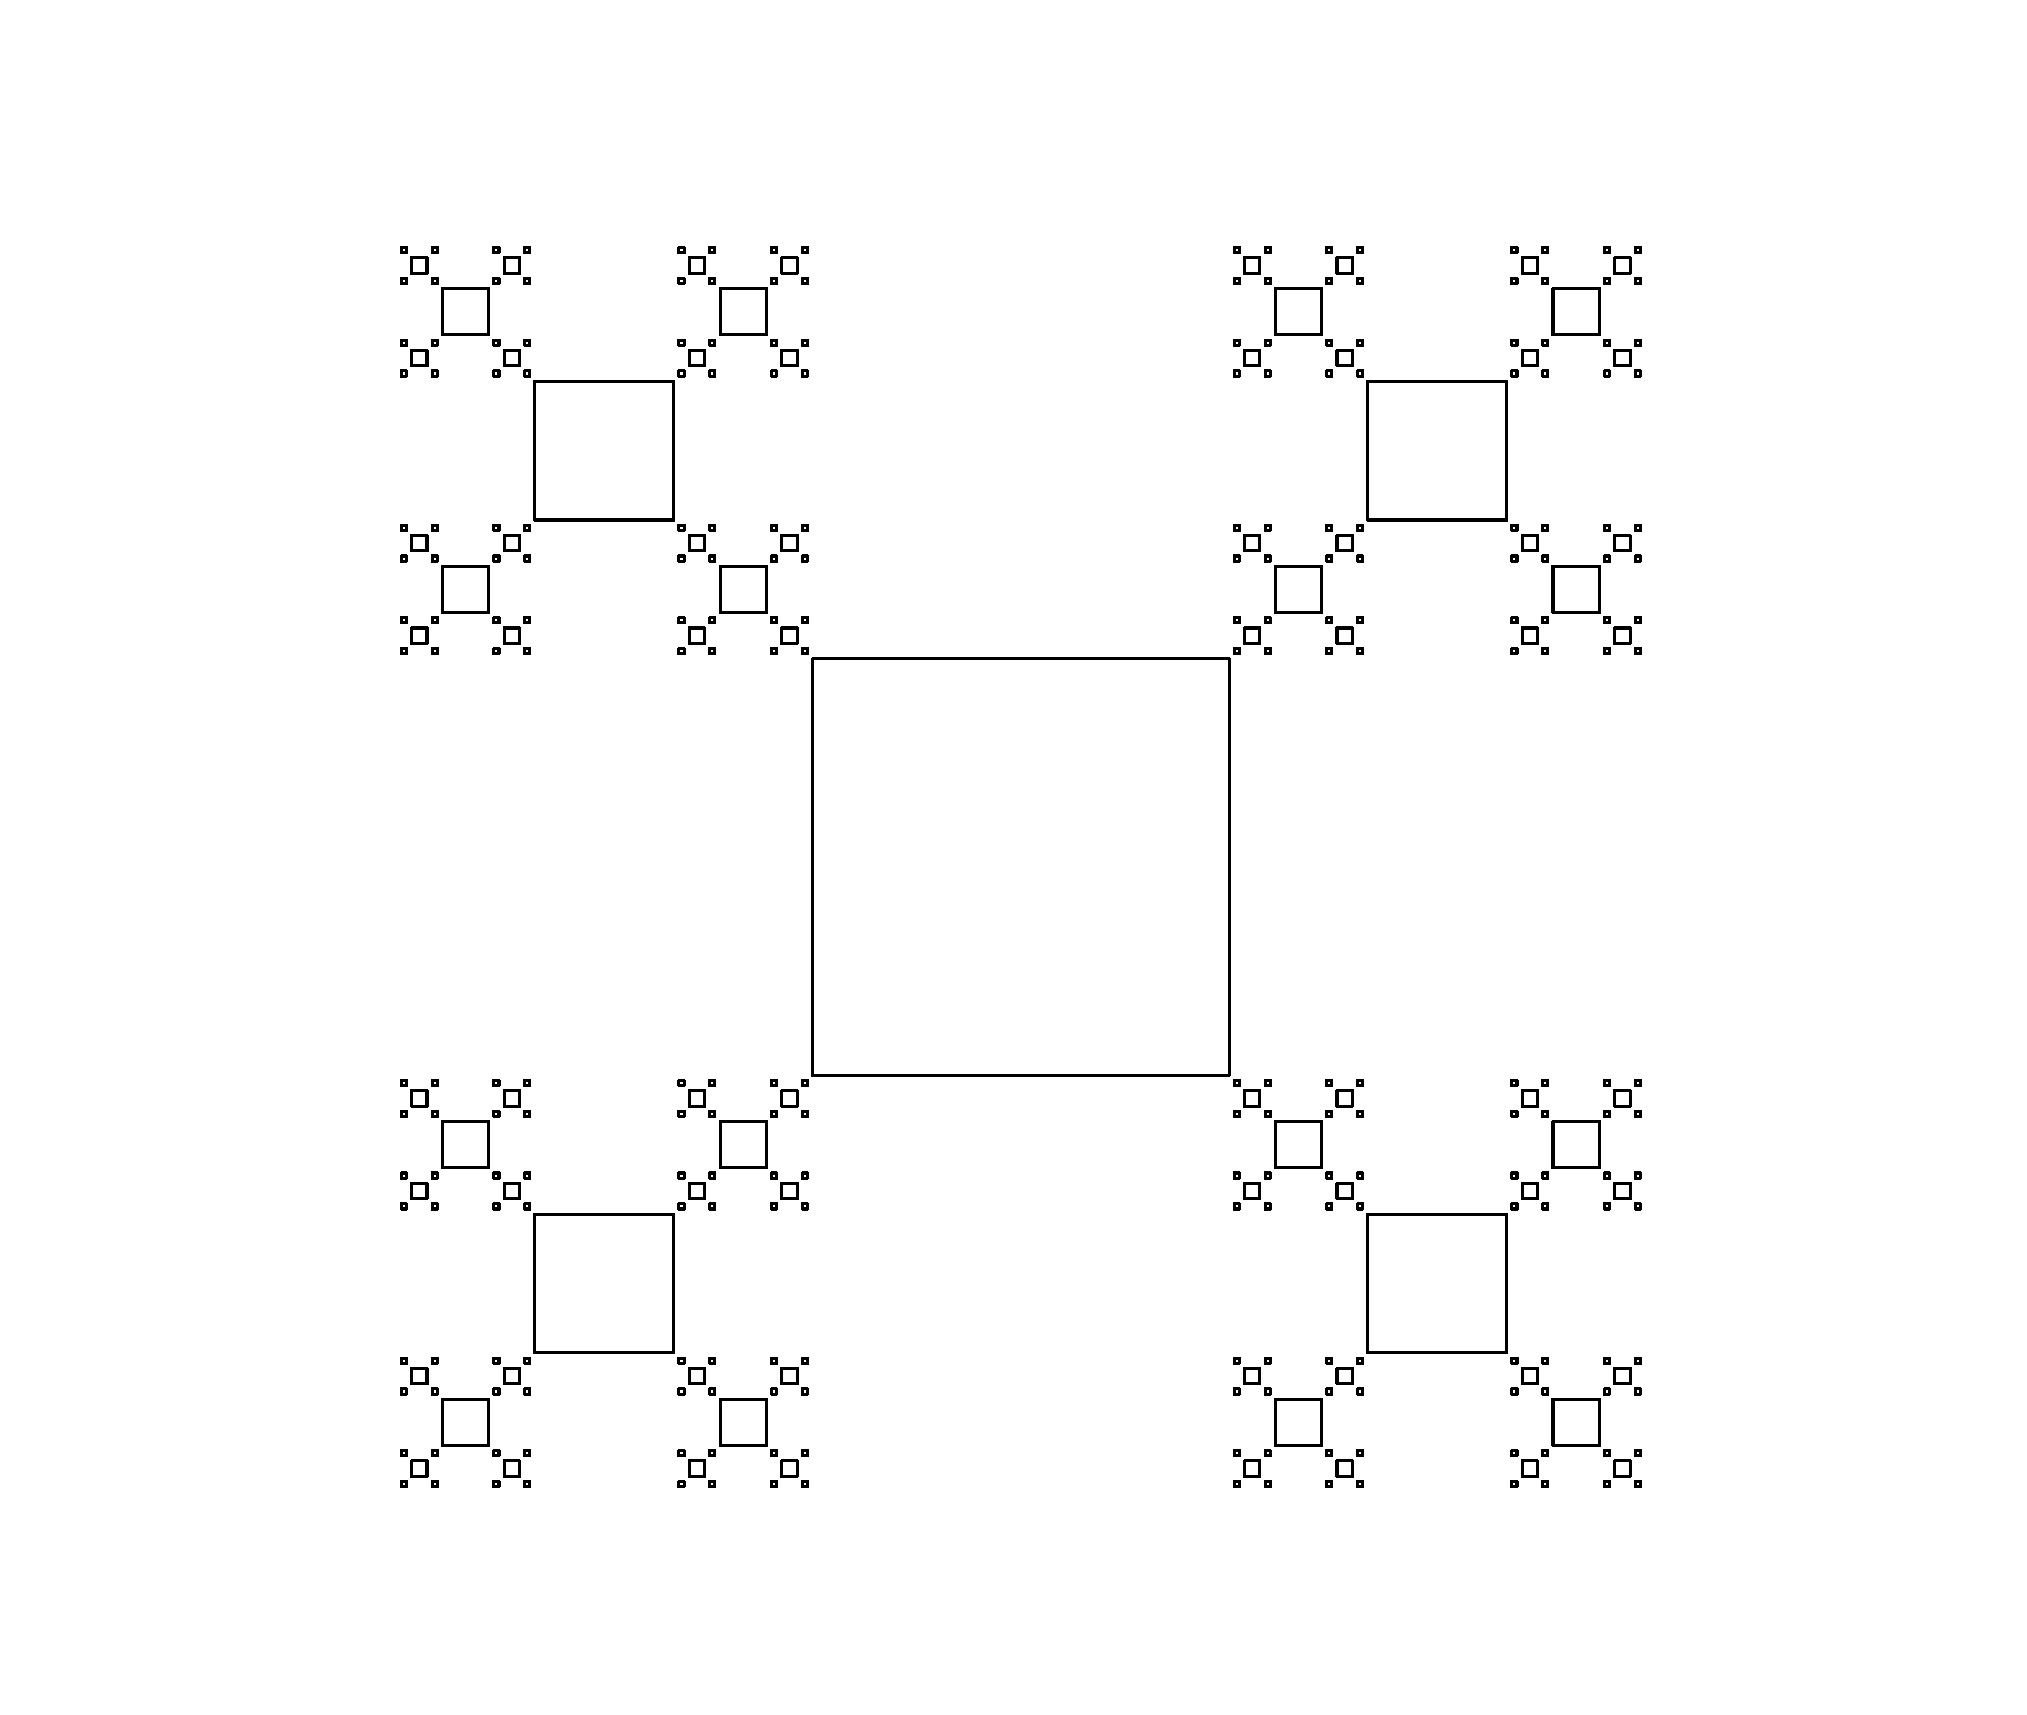
\includegraphics[trim=780 780 780 780,height=10cm]{fractal-200-5.eps}
\end{center}

Per pintar una fractal del poder de $n\ge1$ nivells de mida $m$, cal pintar un quadrat de mida~$m/3$, i quatre fractals del poder a les seves quatre cantonades amb $n-1$ nivells i mides $m/3$. Una fractal de zero nivells és buida.

\bigskip

Per exemple, aquestes són les fractals del poder amb 0, 1, 2, 3, 4, i 5 nivells:

\begin{center}
0 ~
\fbox{

\includegraphics[trim=780 780 780 780,height=3.5cm]{fractal-200-0.eps}
}
\qquad
1 ~
\fbox{

\includegraphics[trim=780 780 780 780,height=3.5cm]{fractal-200-1.eps}
}
\qquad
2 ~
\fbox{
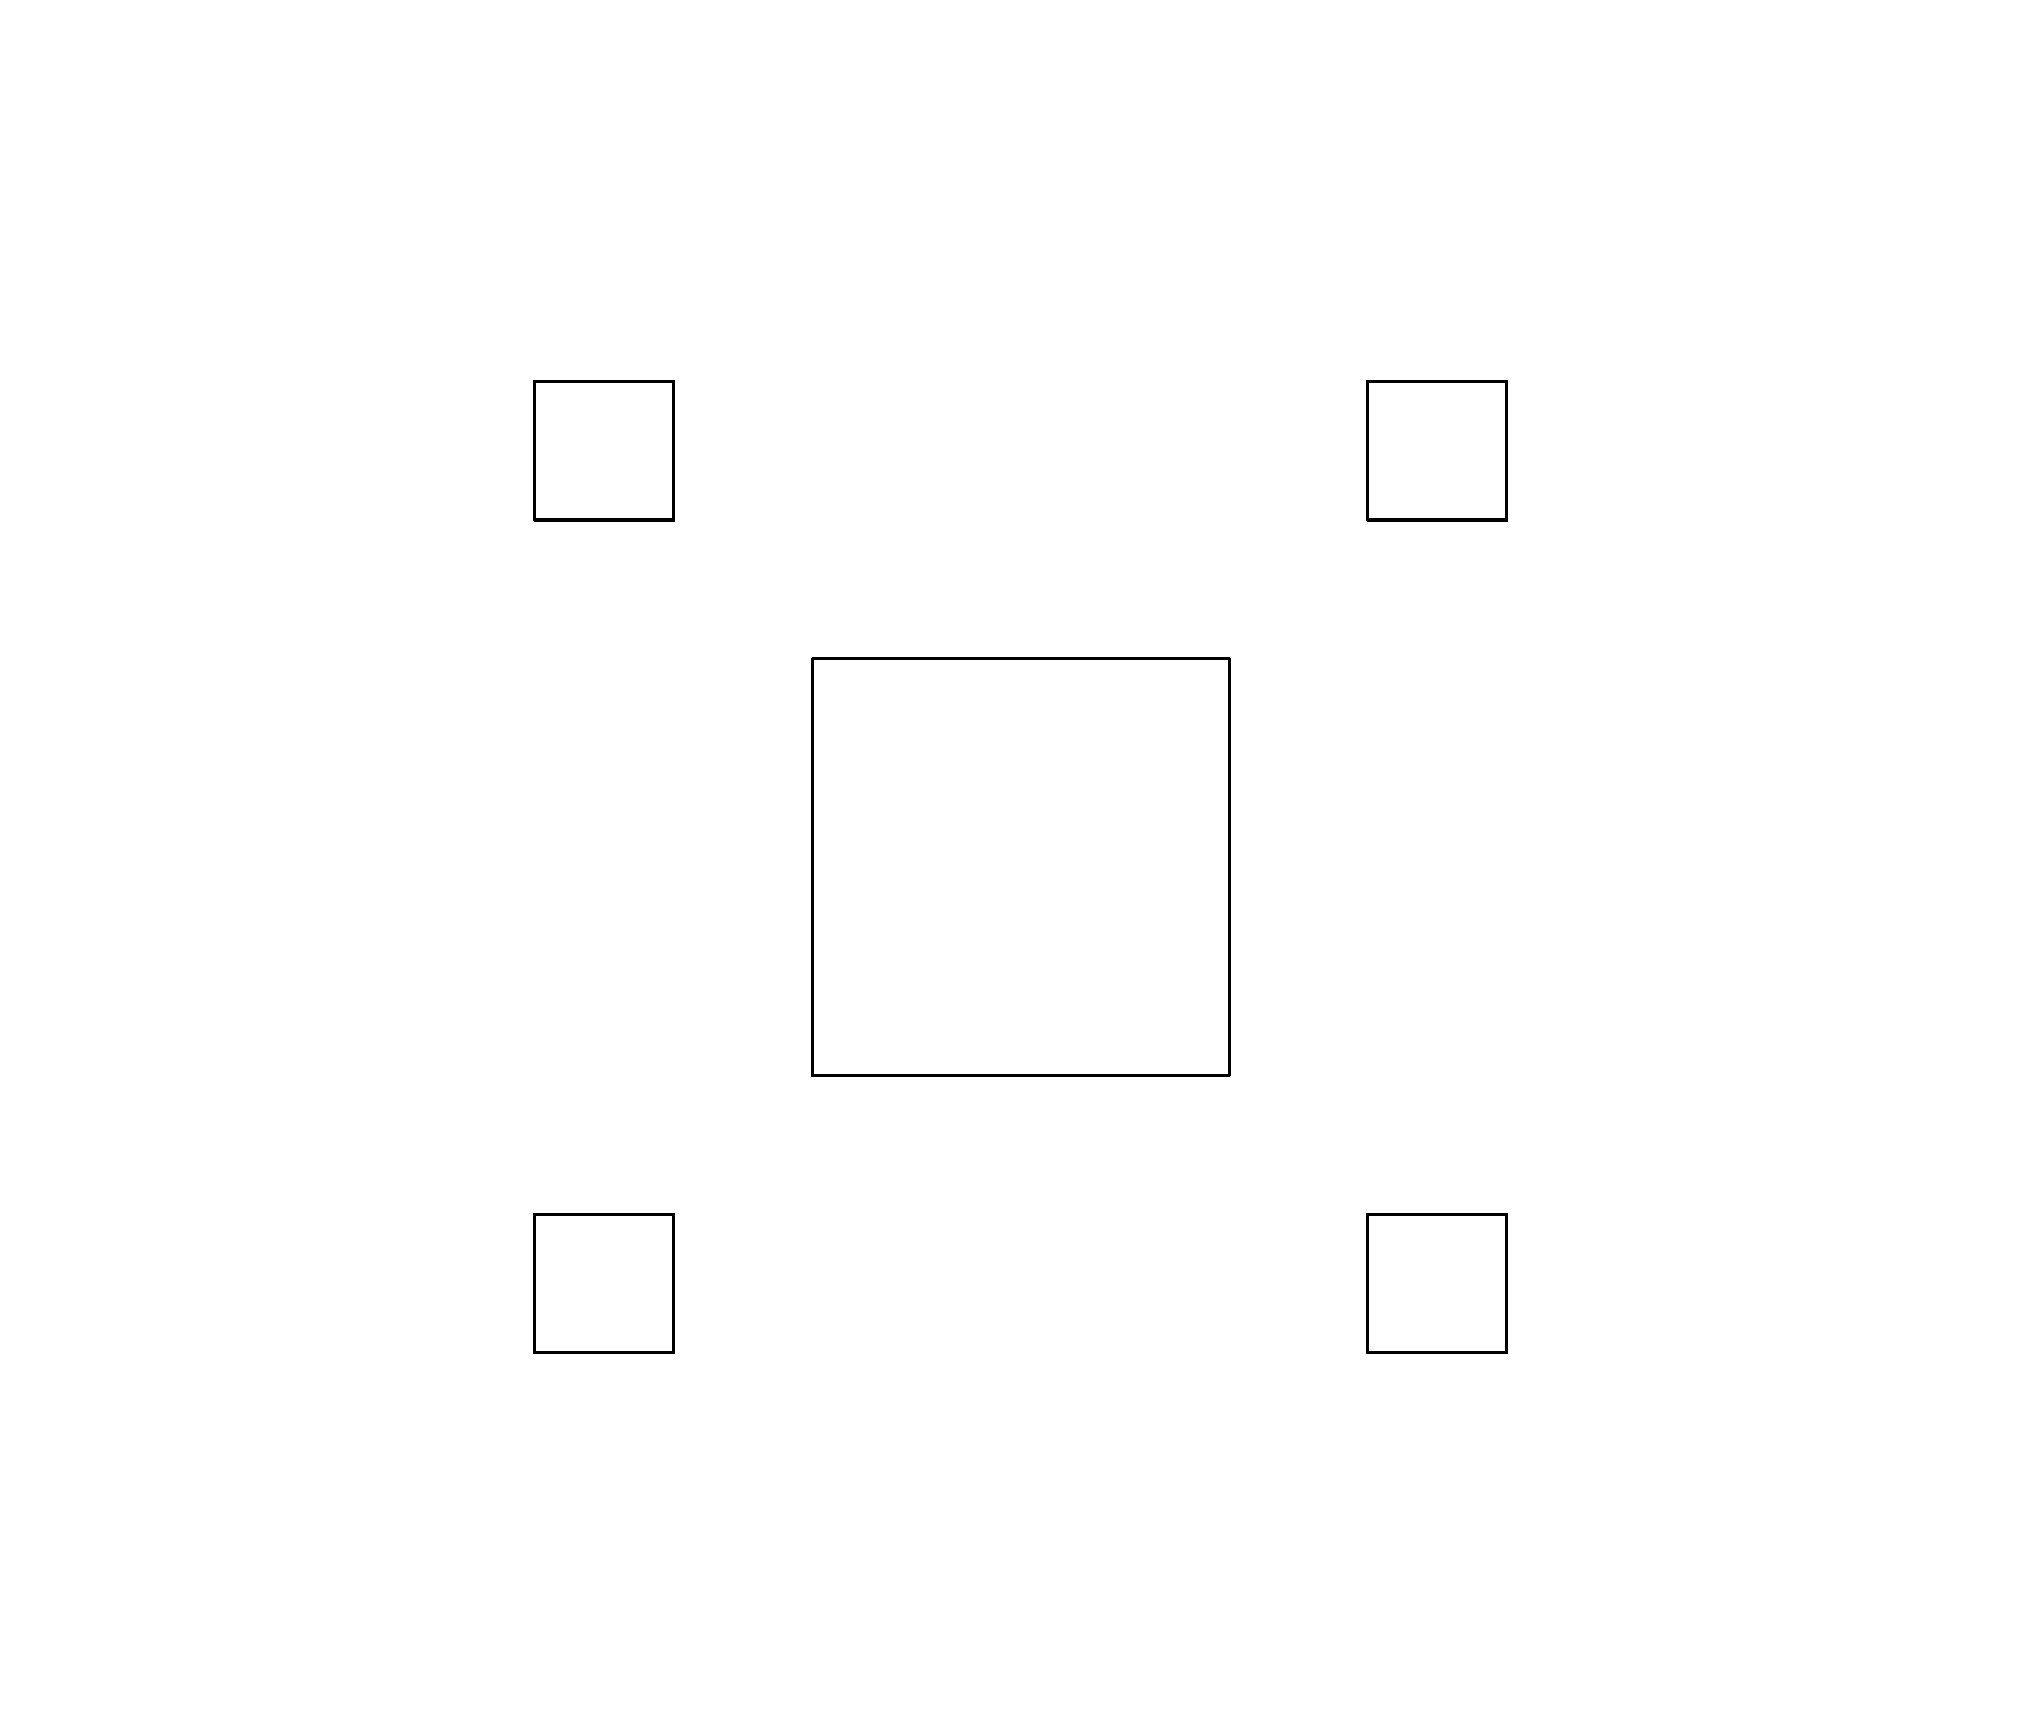
\includegraphics[trim=780 780 780 780,height=3.5cm]{fractal-200-2.eps}
}

\bigskip
\bigskip

3 ~
\fbox{
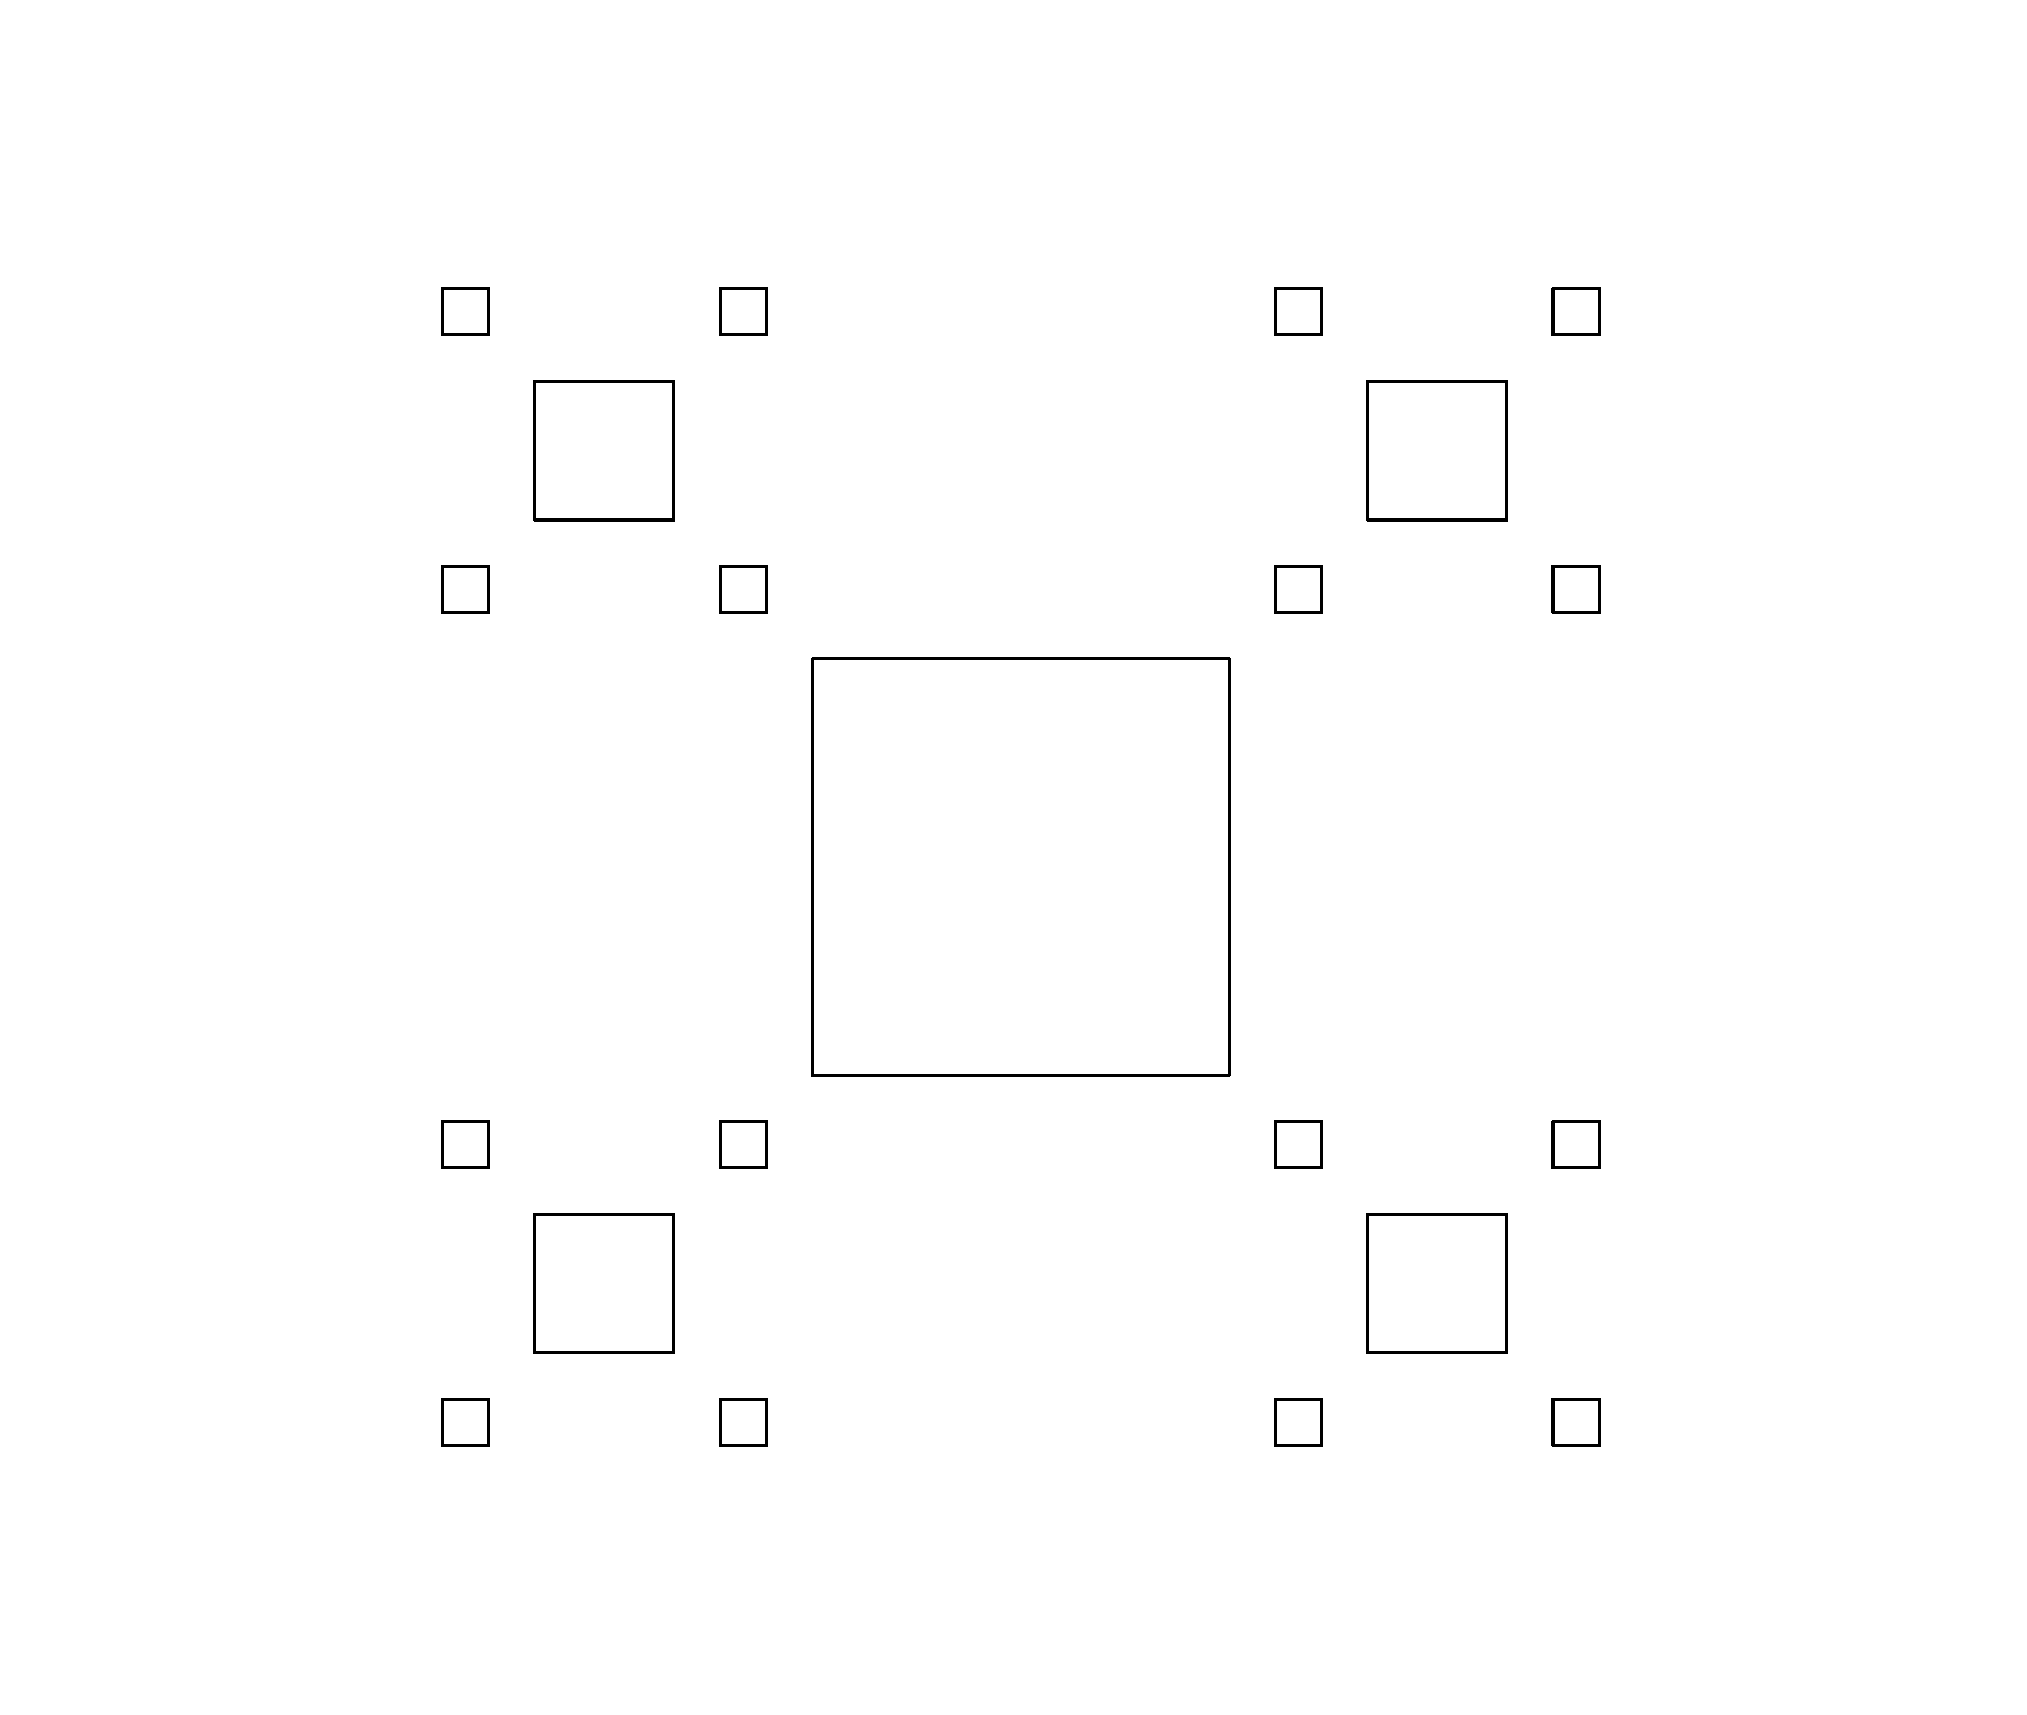
\includegraphics[trim=780 780 780 780,height=3.5cm]{fractal-200-3.eps}
}
\qquad
4 ~
\fbox{
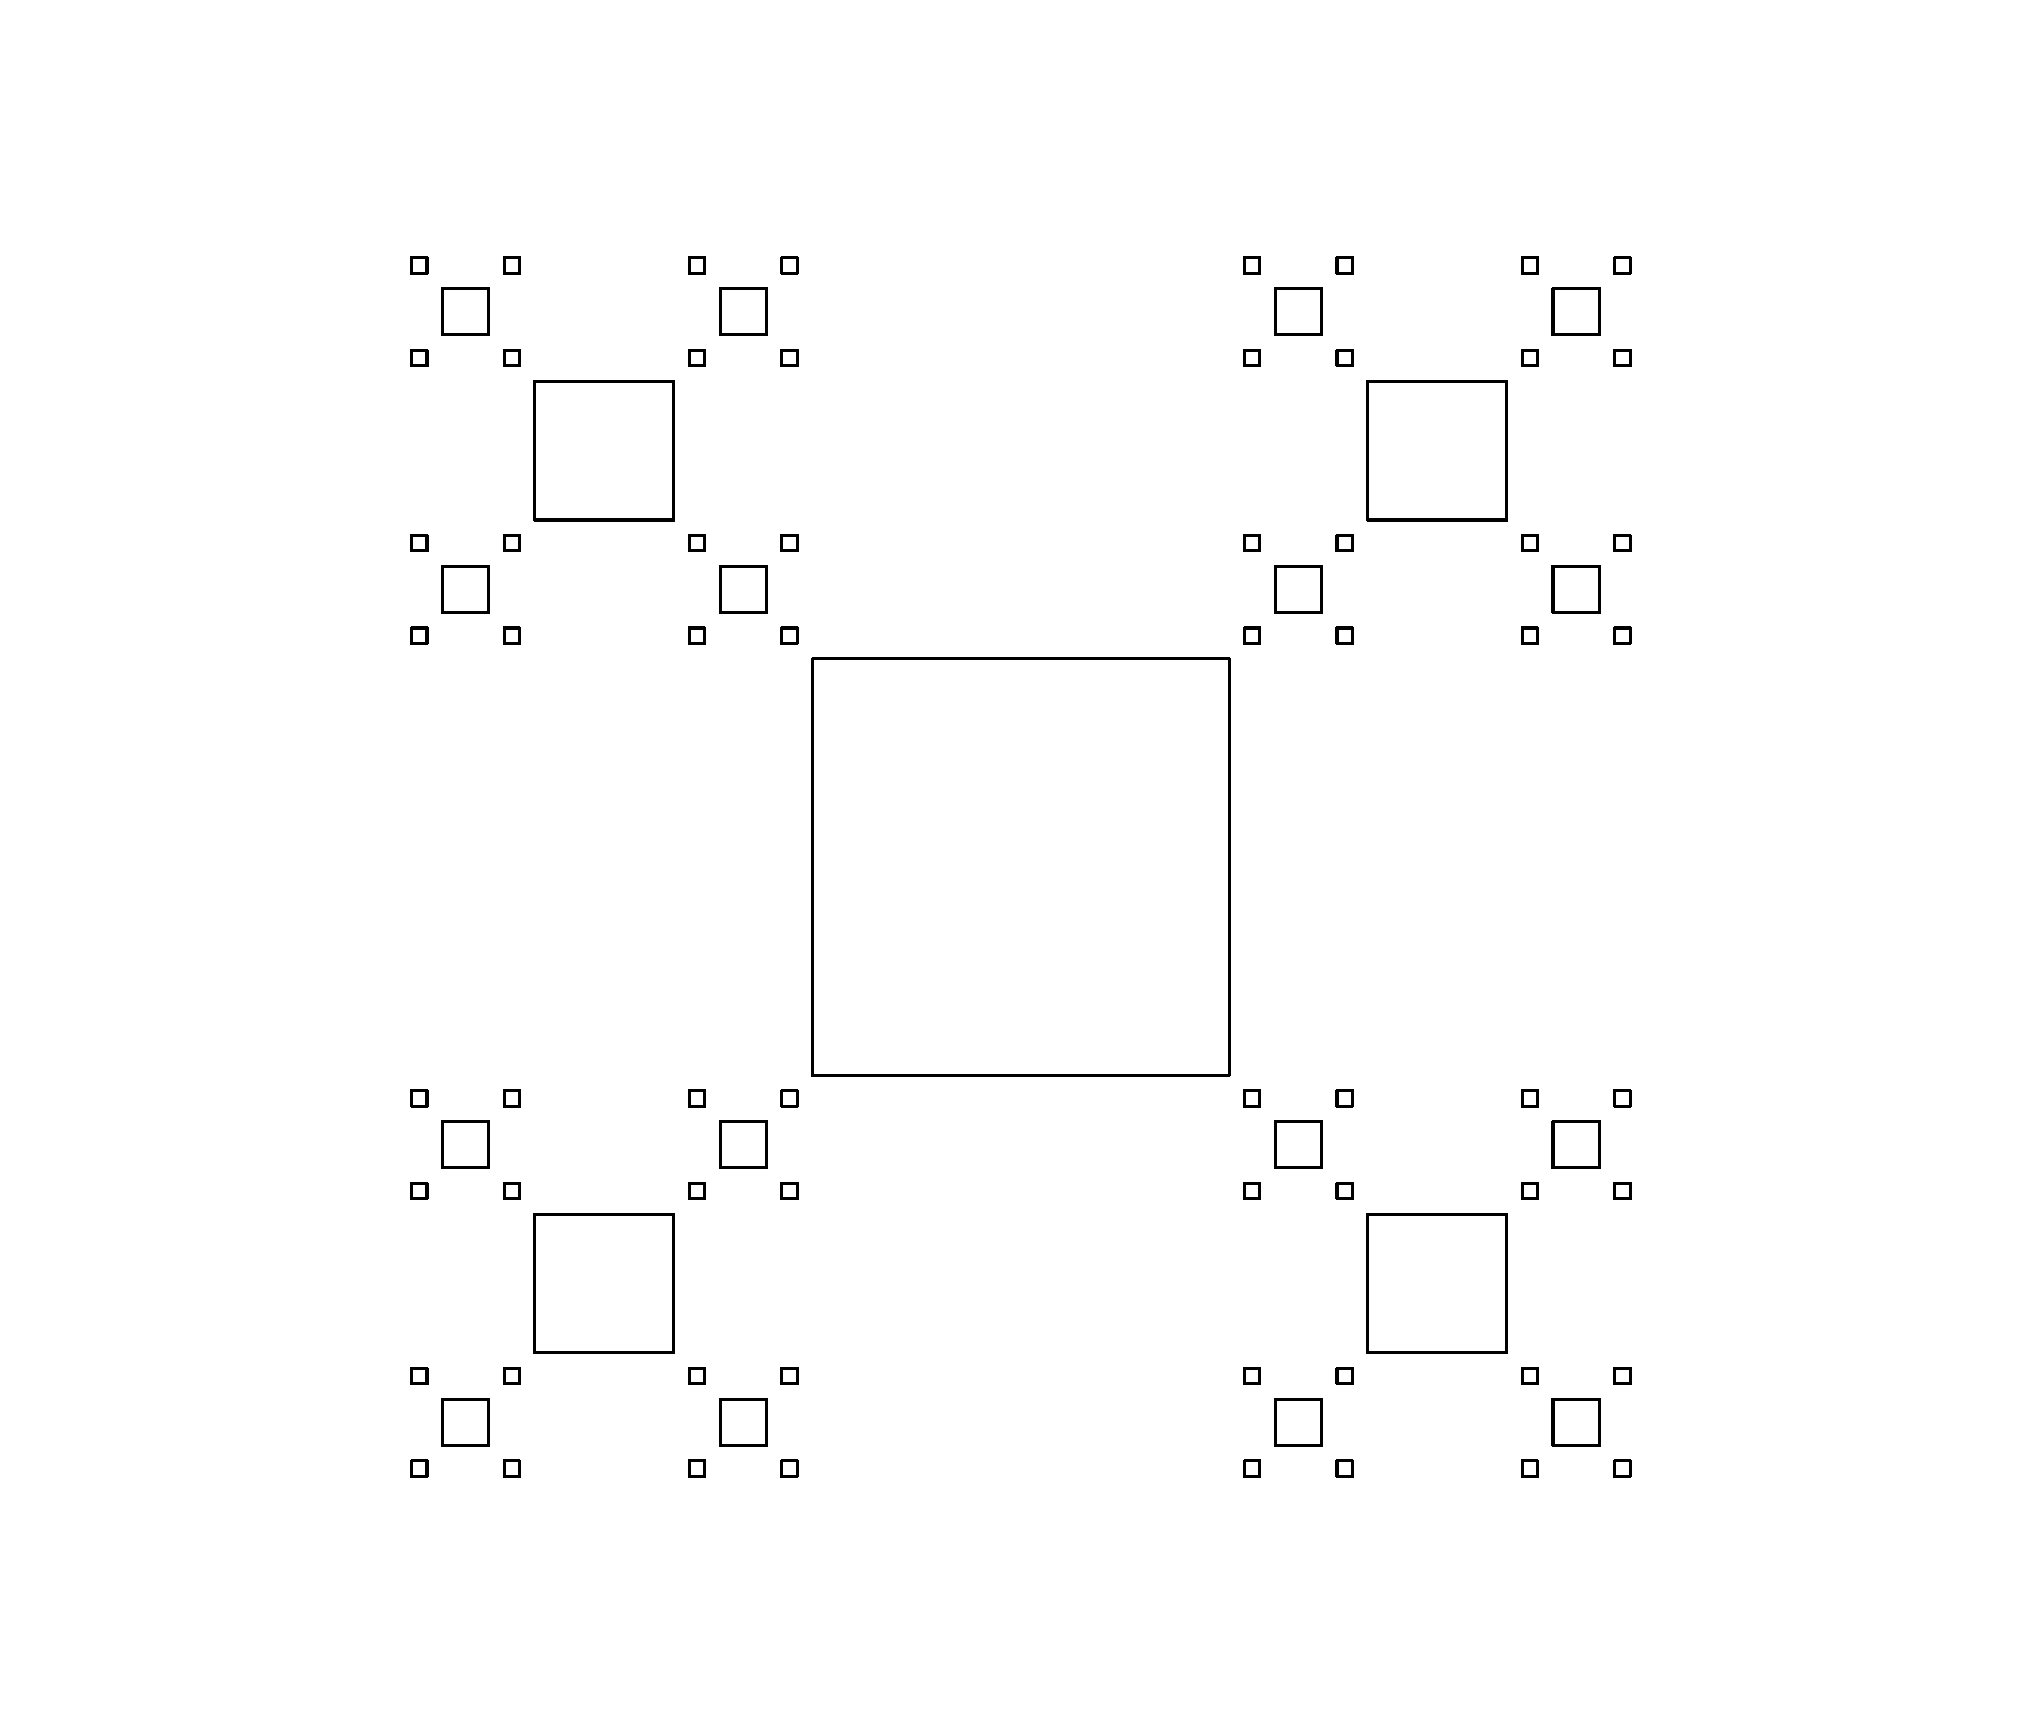
\includegraphics[trim=780 780 780 780,height=3.5cm]{fractal-200-4.eps}
}
\qquad
5 ~
\fbox{
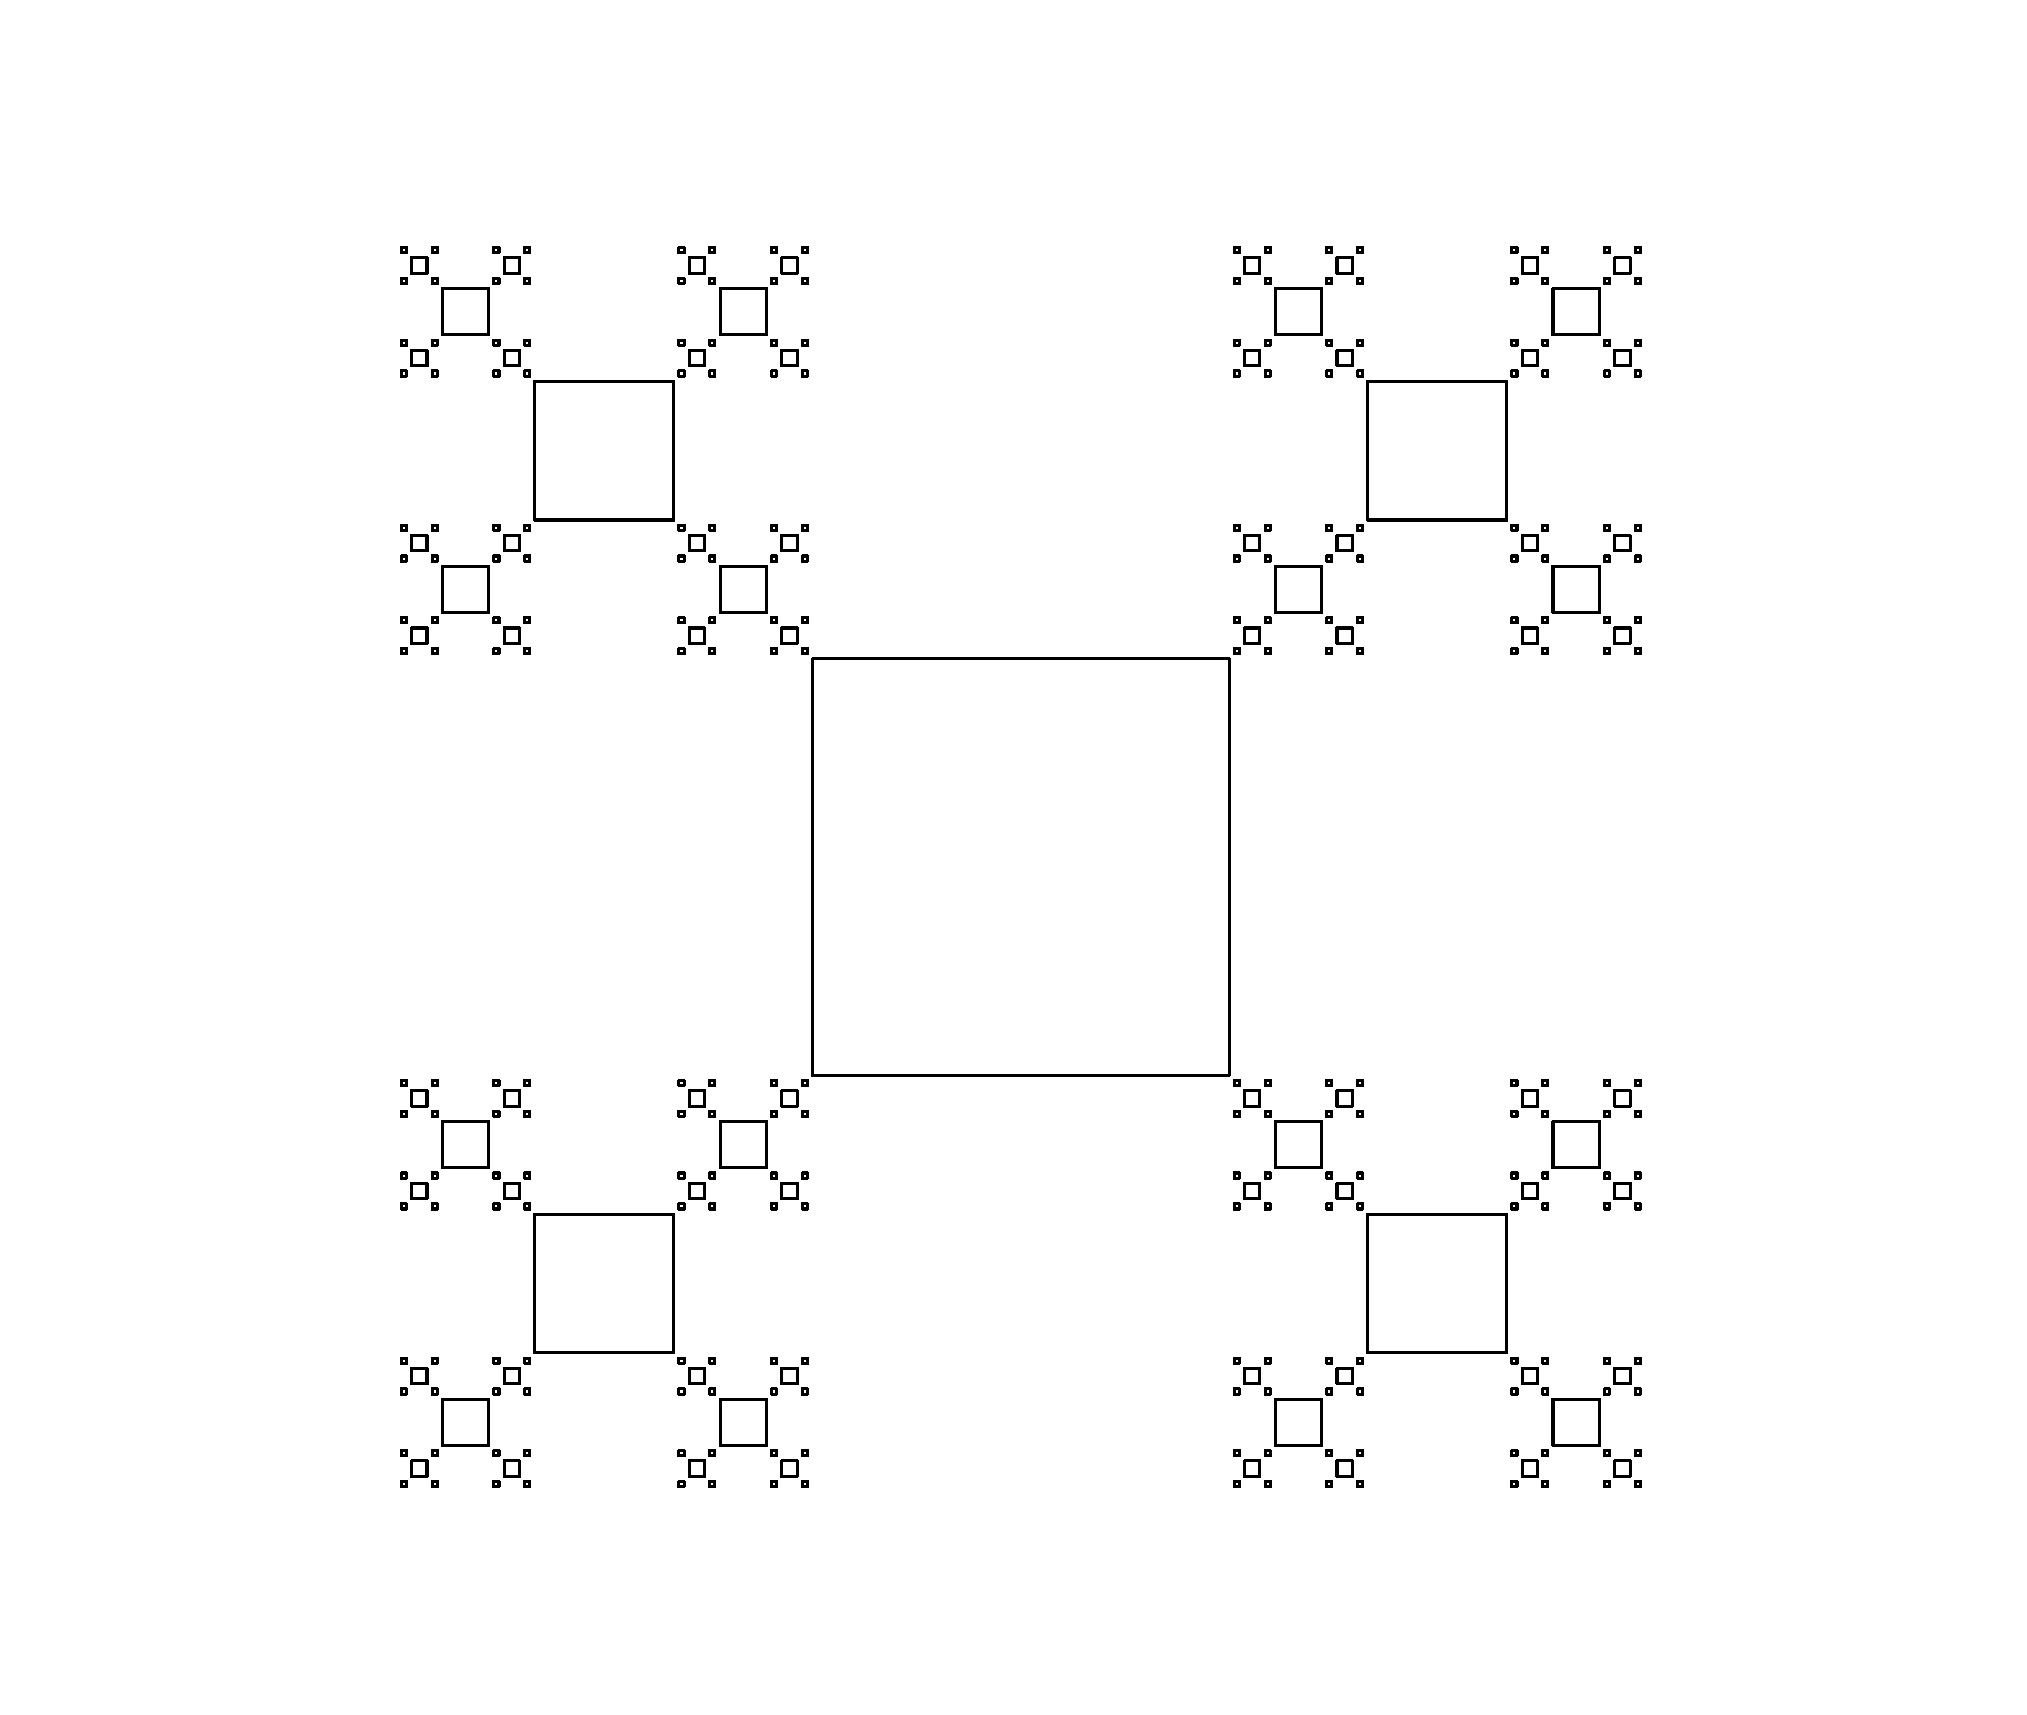
\includegraphics[trim=780 780 780 780,height=3.5cm]{fractal-200-5.eps}
}
\end{center}

\mysection{Entrada}

A l'entrada, es donen dos valors: un real positiu $m$ amb la mida de la fractal i un natural $n$ amb el seu nombre de nivells.

\mysection{Sortida}

El programa ha de dibuixar la fractal del poder d'$n$ nivells i
mida $m$ centrada a la finestra.

\bigskip

\begin{multicols}{2}\raggedcolumns
\mysection{Exemple d'entrada 1}

\begin{verbatim}
100
2
\end{verbatim}

\columnbreak

\mysection{Exemple de sortida 1}

\fbox{
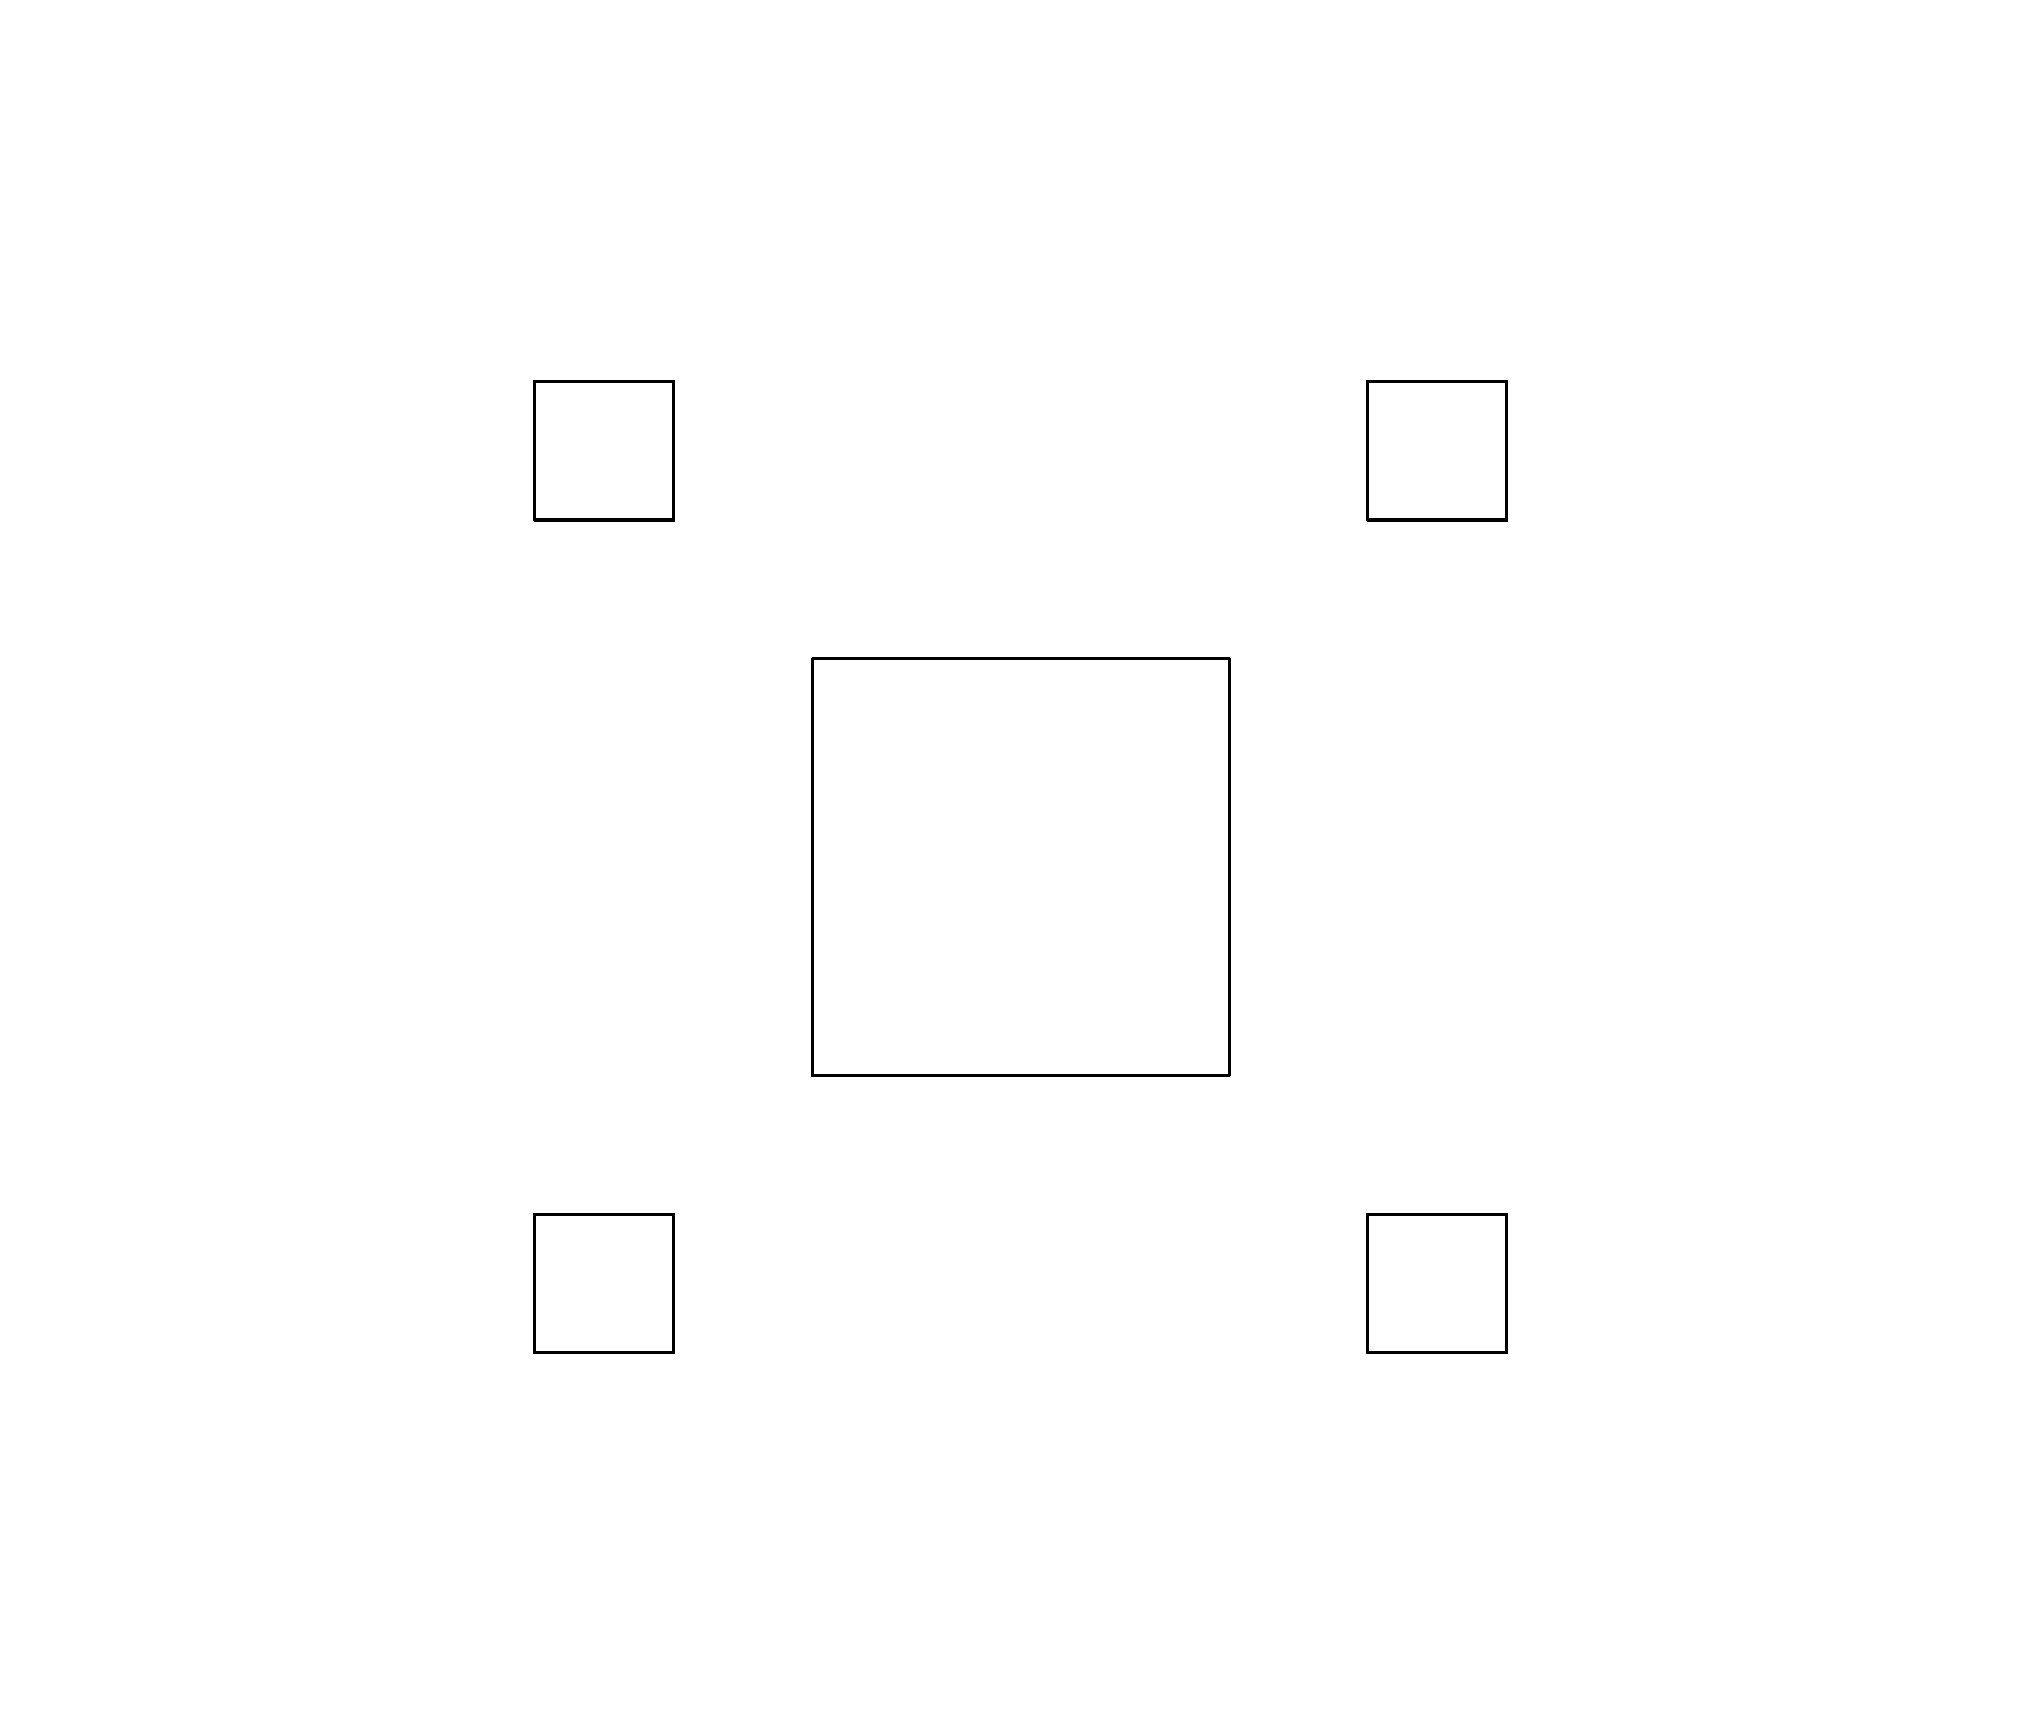
\includegraphics[trim=780 780 780 780,height=3.5cm]{sample1.eps}
}

\end{multicols}

\begin{multicols}{2}\raggedcolumns
\mysection{Exemple d'entrada 2}

\begin{verbatim}
100 3
\end{verbatim}


\columnbreak
\mysection{Exemple de sortida 2}

\fbox{
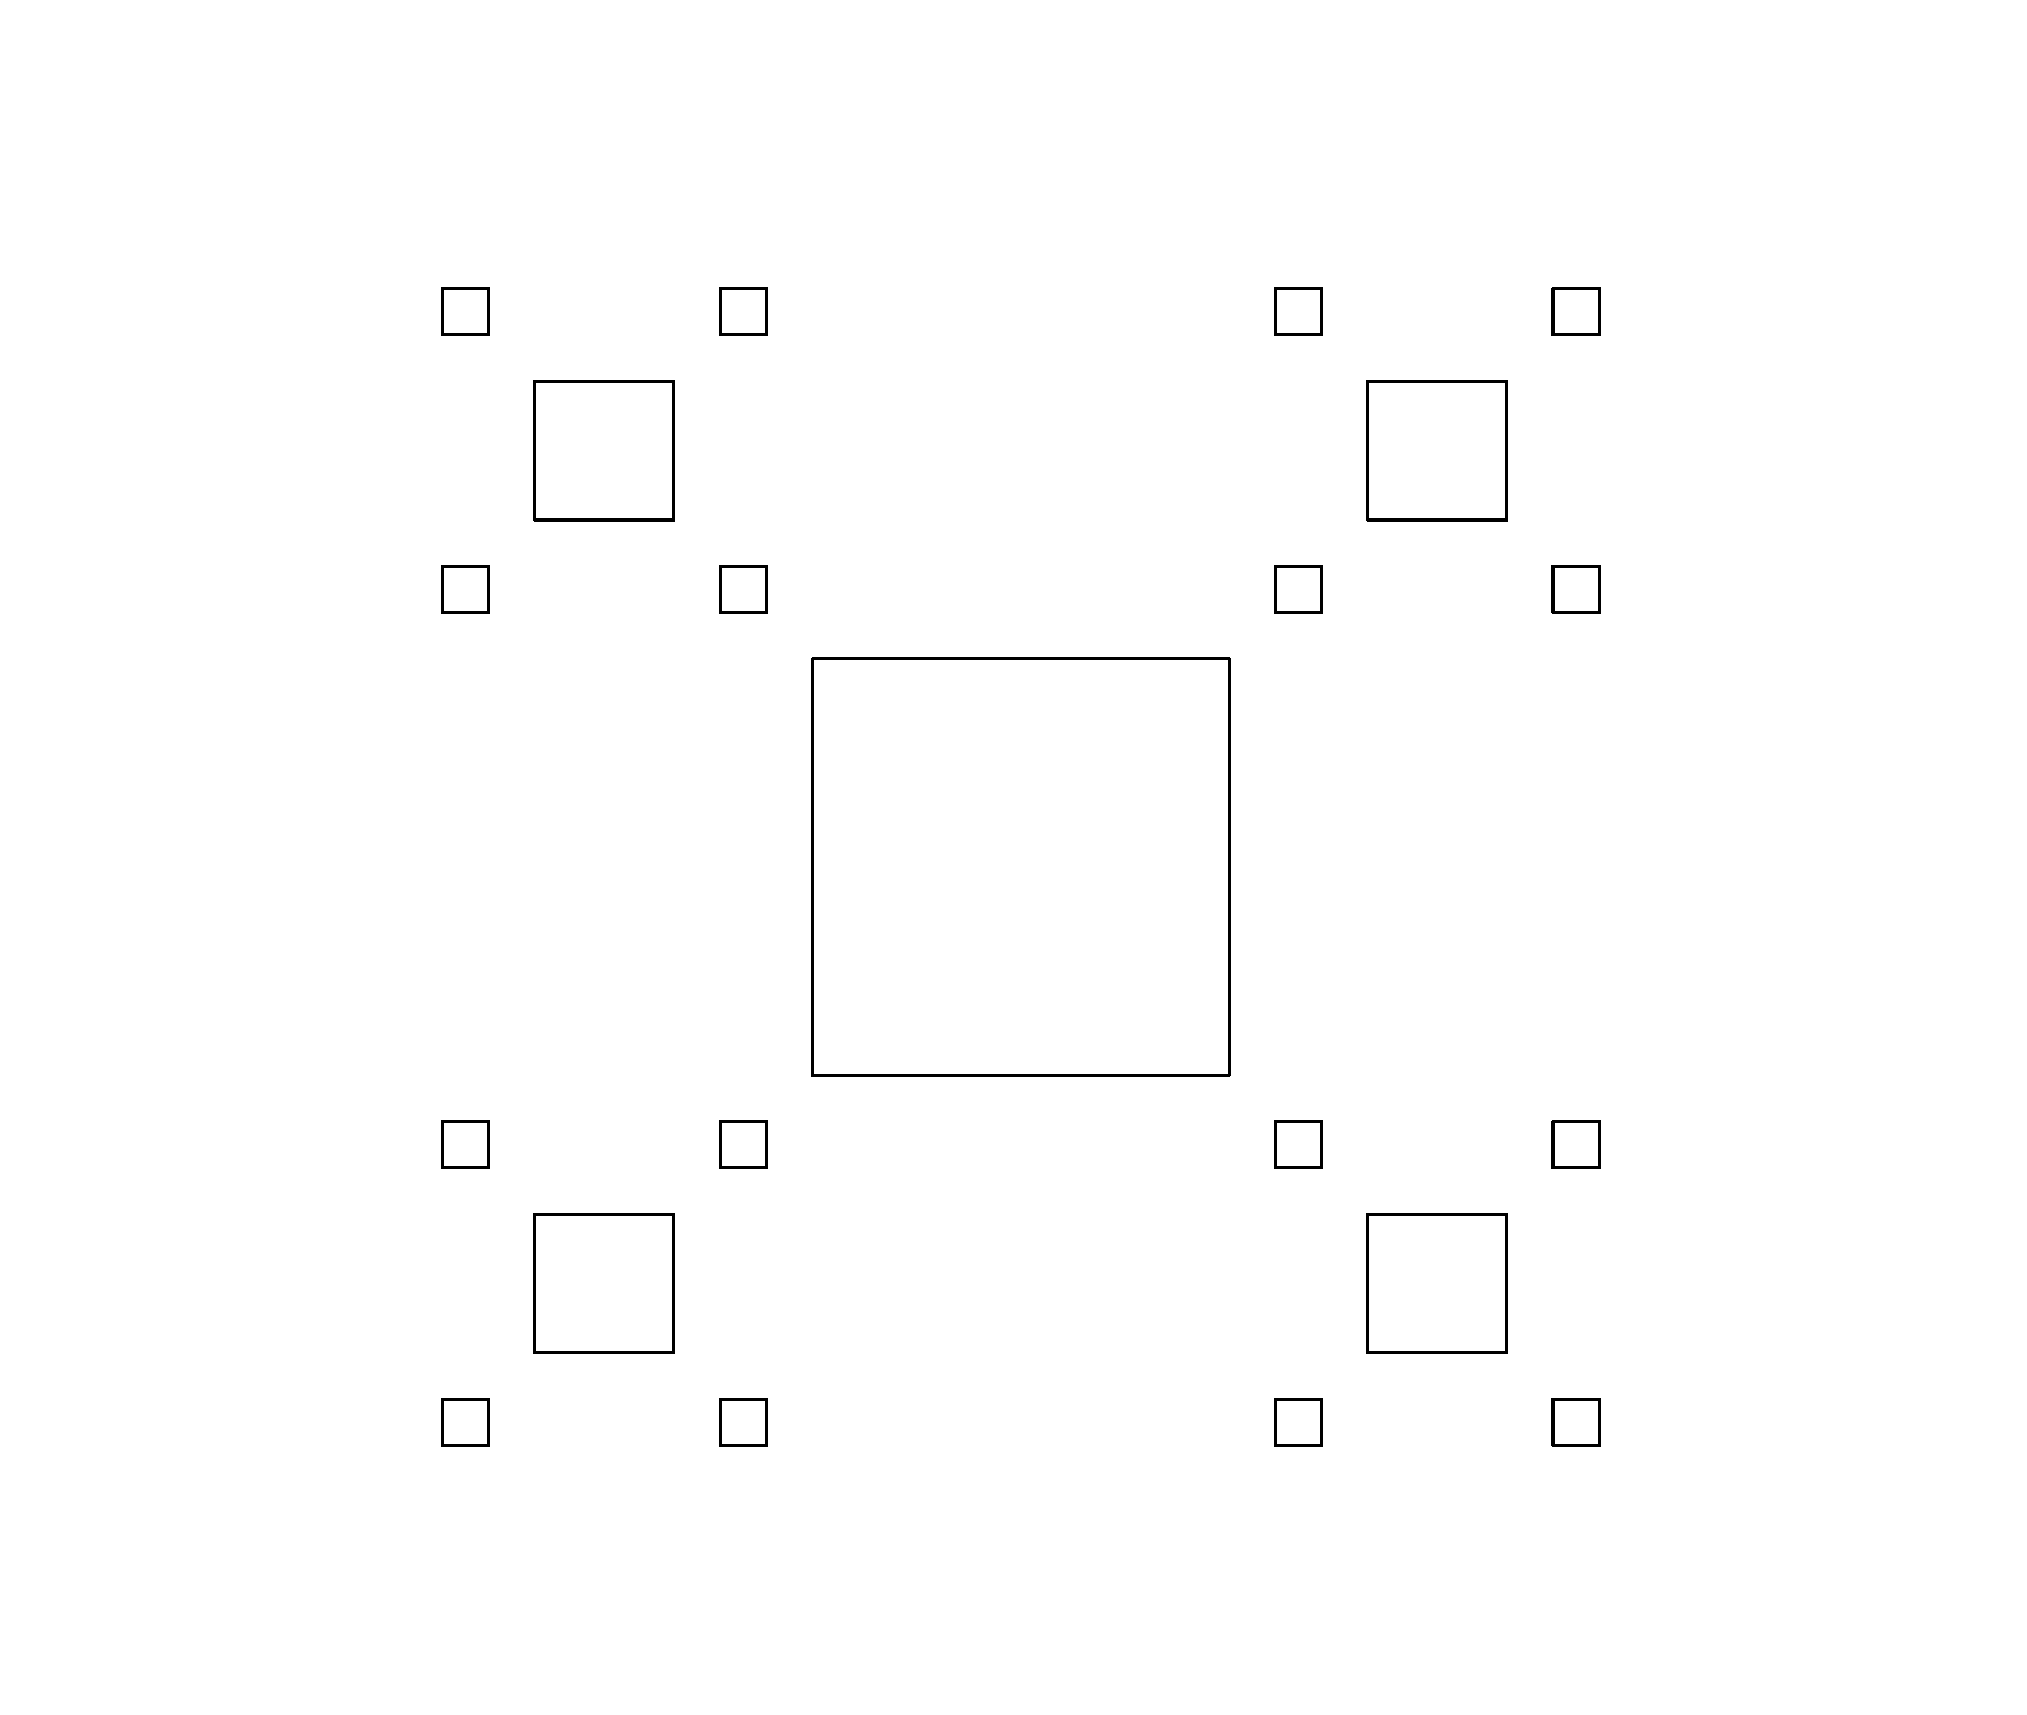
\includegraphics[trim=780 780 780 780,height=3.5cm]{sample2.eps}
}

\end{multicols}


\mysection{Recordatori}

Recordeu que Python ofereix un mòdul \texttt{turtle} que permet pintar images.
Les úniques operacions que us calen són
\texttt{turtle.goto(x, y)} que mou la tortuga a les coordenades (\texttt{x},\texttt{y}),
\texttt{turtle.forward(d)} que avança la tortuga \texttt{d} unitats,
\texttt{turtle.left(a)} que gira la tortuga \texttt{a} graus cap a l'esquerra,
\texttt{turtle.down()} que activa el traçat i
\texttt{turtle.up()} que desactiva el traçat. 
També podeu usar \texttt{turtle.speed(0)} i 
\texttt{turtle.hideturtle()} per fer accelerar la tortuga.
I no oblideu \texttt{turtle.done()} al final del programa. 


\mysection{Important}

No us preocupeu si teniu lleugeres diferències amb els exemples.
